\documentclass[a4paper,10pt]{article}
\usepackage{graphicx}
\usepackage[english]{babel}
\usepackage{subcaption}
\usepackage[latin1]{inputenc}
\usepackage[numbers]{natbib}
\usepackage{amsmath}
\usepackage{float} %for figure formatting
\bibliographystyle{unsrtnat}
\usepackage[top=1.5cm,bottom=2.5cm, left=2.5cm, right=2.5cm]{geometry}
\usepackage{siunitx}
\usepackage[parfill]{parskip}
\usepackage{multirow, amssymb, multicol}
\setlength{\parskip}{1em}

\usepackage{hyperref}
\hypersetup{
    colorlinks,
    citecolor=black,
    filecolor=black,
    linkcolor=black,
    urlcolor=black
}


\begin{document}

\begin{center}
    {\textbf{\Large{Advanced Propulsion notes}}}\\[0.2cm]
    {\large{Cooper Chang Chien}}
\end{center}

\tableofcontents
\newpage


%%%%%%%%%% Main content %%%%%%%%%%
\section{Governing equations of gasdynamics}
Consider an arbitrary pipe with non-constant cross sectional area. Assume (1) no heat loss through walls (2) no external work done by fluid (3) pipe is stationary (4) friction is negligible. 
\begin{gather*}
    \rho_1U_1A_1 = \rho_2U_2A_2\\
    \rho_1U_1^2A_1+P_1A_1=\rho_2U_2^2A_2+P_2A_2\\
    h_1+\frac{1}{2}U_1^2=h_2+\frac{1}{2}U_2^2
\end{gather*}

\subsection{Case A: no losses (isentropic relations)}
Requires: (a) no heat flux through walls, (b) no work done by/to fluid (c) No losses in fluid ($s=$constant)
\begin{gather*}
    \frac{T_0}{T}=1+\frac{\gamma-1}{2}M^2\hspace*{0.5cm}\frac{P_0}{P}=\Big(1+\frac{\gamma-1}{2}\Big)^{\frac{\gamma}{\gamma-1}}\hspace*{0.5cm}\frac{\rho_0}{\rho} = \Big(1+\frac{\gamma-1}{2}\Big)^{\frac{1}{\gamma-1}}\\[0.15cm]
    \frac{A}{A^*}=\frac{1}{M}\Big[\frac{2}{\gamma-1}\Big(1+\frac{\gamma-1}{2}M^2\Big)\Big]^{\frac{\gamma+1}{2(\gamma-1)}}
\end{gather*}

\subsection{Case B: losses allowed}
If we allow change in entropy (i.e. Q through the wall) and we take two stations on the pipe so that the surface area between is small so that $Q$ is negligible. Prior to analysis, note that regardless of losses, \textbf{momentum and mass must still be conserved}.
\begin{gather*}
    \frac{P_2}{P_1} = \underbrace{\frac{1+\gamma M_1^2}{1+\gamma M_2^2}}_\text{momen. con} = \underbrace{\frac{M_1}{M_2}\sqrt{\frac{T_2}{T_1}}}_\text{mass con} = \underbrace{\frac{M_1}{M_2}\sqrt{\frac{1+\frac{\gamma-1}{2}M_1^2}{1+\frac{\gamma-1}{2}M_2^2}}}_\text{no stagn. T losses}\\
    \boxed{M_2=\sqrt{\frac{(\gamma-1)M_1^2+2}{2\gamma M_1^2-(\gamma-1)}}}
\end{gather*}
The above equation presents the possibility of a step change in Mach number, which indicates a discontinuity (\boxed{\textbf{SHOCK}}) \textbf{MUST} happen. Only if the discontinuity happens, the relation holds by necessarily require $M_1>1$ (supersonic inlet flow), assuming no heat flux through walls. 



\section{Diffuser (M 0.8$\rightarrow$2)}
A presence of a body causes subsonic flow field diffusion upstream via propagation of pressure fields. For supersonic flow fields, the information cannot propagate fast enough. In order to slow to flow to subsonic when reached the compressor, a normal shock can be used. However, a shock can be inefficient causing large losses in $P_0$ ($M_1=2$, loss $\approx20\%$). Therefore, the \textbf{position of a normal shock} is important. 

\subsection{Converging-Diverging inlet diffuser (normal shock)}
The importance in this type of diffuser is how to sustain the normal shock position at the optimal placement and minimise the loss. The optimal operating point is where the \textbf{normal shock is just passed the throat} when the shock mach number is just over 1, with minimal losses. (just after T in Figure \ref{fig:diffuser})

If a stand-off shock is formed (1 in Figure \ref{fig:diffuser}), this is due to the diffuser is operating at off-design conditions. In order to "swallow" the normal shock to the inlet of the diffuser and further down to the optimal position, there's two ways to do so: (Assuming flight mach number = 1.4)

\subsubsection{Overspeed}
If we assume the area $A_2/A_T$ is fixed, the condition are constrained at (1) by the normal shock, therefore the mass flow rate (or capture area) $A_1\neq A_2$, inducing mass flow lost. 
\begin{gather*}
    @M=1.4,\hspace*{0.4cm}\boxed{\frac{A_2}{A_T} = 1.1149},\hspace*{0.5cm}\text{After shock @ 1, }M_1=0.7397,\hspace*{0.3cm}\boxed{\frac{A_1}{A_T} = 1.0681}
\end{gather*}
In order to match the difference in area ratio, requires overspeed to "swallow" (or get shock to station 2) to increase $M_\infty$ until $A_1/A^* = 1.1149=A_2/A_T$. The losses in mass flow rate and the overspeed ratio required can be calculated as follow:
\begin{gather*}
    \frac{\dot{m}}{\dot{m}_{design}} = \frac{\rho_1}{\rho_\infty}\sqrt{\frac{T_1}{T_\infty}}\frac{M_1}{M_\infty}\frac{A_1}{A_T}\frac{A_T}{A_2},\hspace*{0.7cm}R_{overspeed} = \frac{M_\infty^{\prime}}{M_\infty}
\end{gather*}
\begin{figure}[H]
    \centering
    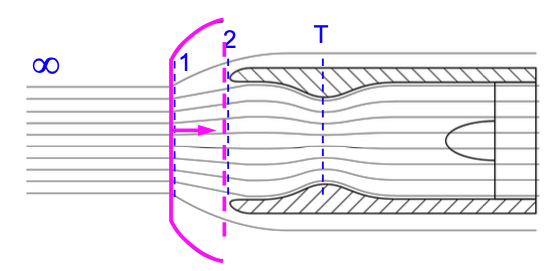
\includegraphics[width=0.5\textwidth]{Figure/diffuser.png}
    \caption{diffuser}
    \label{fig:diffus  er}
\end{figure}
\vspace*{-0.3cm}
\underline{\textbf{NOTE:}} NOT practical when $M_\infty\approx1.8$.

\subsubsection{Variable geometry inlet}
Alternatively, we can vary $A_T$ that would choke an area $A_2$ at the conditions at station (1). If we now assume that the condition at station 1 is are new $A_2$
\begin{gather*}
    \frac{A_T^{\prime}}{A_T} = \frac{A_2}{A_T}\frac{A_T^{\prime}}{A_2}
\end{gather*}


\subsection{Spike diffuser (Mach Wave)}
a very thin spike extends upstream of the engine inlet. A Mach wave forms off the tip and designed so that the oblique shock hits the edge of the engine nacelle (A spike will generate an oblique shock even with ramp angle $\delta\rightarrow0$). However, pressure compression is nearly negligible.
\begin{gather*}
    \sigma = \sin^{-1}\Big(\frac{1}{M_1}\Big),\hspace*{0.8cm}\frac{P_2}{P_1}=\frac{2\gamma}{\gamma+1}M_1^2\sin^2\Big(\underbrace{\sin^{-1}\frac{1}{M_1}}_\sigma\Big)-\frac{\gamma-1}{\gamma+1} = 1
\end{gather*}

\subsection{Oblique shock diffuser}
Oblique shock diffusers are common on high-speed engine inlets due to the capability of oblique shocks increases capture area (important at high altitudes where density are low). Using a \textbf{succession of many weaker oblique shocks} produces less entropy and minimises $P_0$ loss. A variable geometry spike inlet is also useful to tune different flight conditions. Off-design can induce "overspill:

\begin{figure}[H]
    \centering
    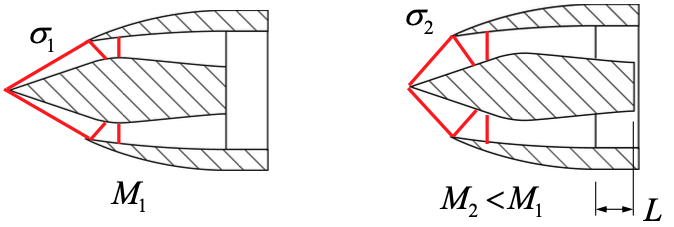
\includegraphics[width=0.5\textwidth]{Figure/os_diffuser.png}
    \caption{oblique shock diffuser}
\end{figure}


\newpage
\section{Combustion/Burner (M 2$\rightarrow$5)}
When operating at $M\approx5$, problems at the combustion starts to show up. The Mach number going into the combustion chamber depends on the ratio of temperatures ($T_2/T_1$) between the inlet and after the diffuser. Constraints on the temperature is mainly from the melting point of existing materials,
\begin{gather*}
    T_1 = 210\text{ K},\hspace*{0.4cm}1500^{\circ}\text{ K}<T_2<2000^{\circ}\text{ K}
\end{gather*}
When the temperature starts to approach $1500^{\circ}$ K, $M_1$ is roughly 5, thus the limitation. 

\subsection{Thermodynamic efficiency $\eta_{th}$}
\begin{gather*}
    \eta_{cycle} = \frac{\text{cycle work}}{\text{heat added}} = 1-\frac{h_4-h_1}{\Delta h_{burn}},\hspace*{0.4cm}\text{where}\hspace*{0.3cm}\Delta h_{burn} = \frac{\dot{m}_f \varepsilon}{\dot{m}_a} = f_{FA}\varepsilon
\end{gather*}
where $f_{FA}$ is the fuel-to-air ratio, and $\varepsilon$ is the heating value of fuel (kJ/kg), by substituting terms,
\begin{gather*}
    \boxed{\eta_{cycle}} = 1-\frac{h_4-h_1}{f_{FA}\varepsilon} = 1-\frac{C_pT_1}{f_{FA}\varepsilon}\Bigg(\frac{T_4}{T_3}\frac{T_3}{T_2}\frac{T_2}{T_1}-1\Bigg) = \frac{C_pT_1}{f_{FA}\varepsilon}\Bigg(\frac{T_2}{T_1}-1\Bigg)\Bigg[\eta_c\eta_e\Bigg(1+\frac{T_1}{T_2}\frac{f_{FA}\varepsilon_1}{C_pT_1}\Bigg)-1\Bigg]
\end{gather*}
Based on the previous assumption assuming there's no shaft work in/out the engine, the best thermo efficiency we can get out fo freestream compression is only 8\%, this is why turbojets need additional mechanical compression. When the flight Mach number reaches around 3, the efficiency without compression component actually exceeds conventional turbojets. 

\begin{figure}[H]
    \centering
    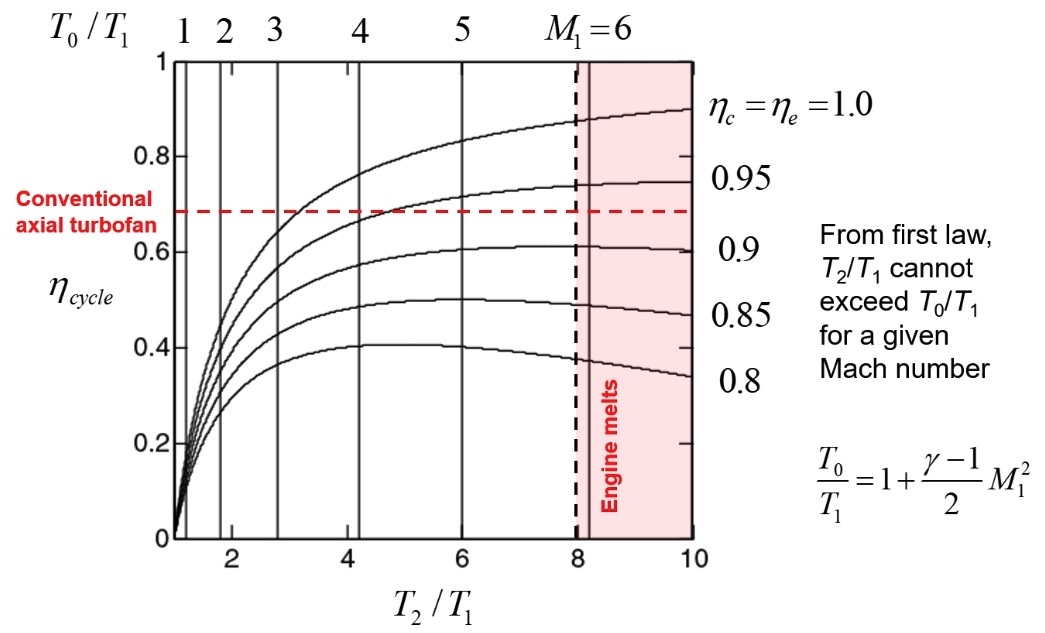
\includegraphics[width=0.6\textwidth]{Figure/burner.png}
\end{figure}

\vspace*{-0.5cm}
\subsection{Subsonic Combustion}
In most cases, the flow needs to be slowed down to about $\boxed{M\approx0.2}$ within the combustion chamber. Combustion is an exothermic chemical reaction with reasonably low activation energy. In order to sustain this exceeded activation energy for the fuel to burn, we need to have \boxed{\textbf{flameholders}} to provide an "anchor" for the reaction to keep place\footnote{This is analogous to blowing out a candle. when blowing a candle, high-speed air blows reaction mix away from the source of fuel. When the heat generated by the reaction is too far, the fuel/air mixture no longer exceeds its activation energy.}. 

\begin{figure}[H]
    \centering
    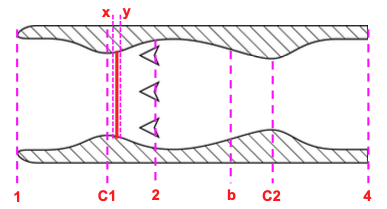
\includegraphics[width=0.45\textwidth]{Figure/ram.png}
    \caption{schematic of ramjet} 
\end{figure}

\subsection{Analysis on Ramjet}
Assume the above ramjet flight condition is $P_1 = 70$ kPa, $T_1=210$ K, and $M_1 = 2.8$

\subsubsection{diffuser (1$\rightarrow$C1)}
Diffuser is an \textcolor{red}{isentropic} process, therefore $T_{01}=T_{0x}$. The pressure and area ratio can be inferred from the isentropic flow $@M=2.8$. The area ratio $A_1/A_{C1}$ provides the throat area required to choke the flow at $M=2.8$.
\begin{gather*}
    \frac{T_{01}}{T_1}=\frac{T_{0x}}{T_1}=2.580,\hspace*{0.4cm}\frac{P_{01}}{P_1}=27.094,\hspace*{0.4cm}\frac{A_1}{A_1^*} = \frac{A_1}{A_{C1}} = 3.485
\end{gather*}

\vspace*{-0.3cm}
\subsubsection{normal shock (x$\rightarrow$y)}
Across the shock, the flow is \textcolor{red}{no longer isentropic}. For minimum $P_0$ loss, the shock strength is set to be really weak as $M_x = 1.1$. The conditions across and after the shock can be found from the 2D normal shock table. \underline{\textbf{NOTE:}} $T_{0x}=T_{01}$, and $A_x = A_y = A_{shock}$
\begin{gather*}
    M_y = 0.912, \hspace*{0.4cm}\frac{P_y}{P_x}=1.245,\hspace*{0.4cm}\frac{\rho_y}{\rho_x}=1.169\\
    \frac{T_{0x}}{T_x} = 1.244,\hspace*{0.4cm}\frac{A_s}{A_{C1}} = 1.008
\end{gather*}

\vspace*{-0.4cm}
\subsubsection{burner entry (y$\rightarrow$2)}
From post shock to the burner entry, the flow is \textcolor{red}{isentropic}. The burner entry Mach number is also constrained to $M_2=0.2$, therefore, the flow after the shock must decelerate from $M_y = 0.91\rightarrow M_2=0.2$. First, to find the area ratio, we can look at the table $@M_y=0.91$ and $@M_2=0.2$ to find their respective choked area ratio. ($A/A^*$)
\begin{gather*}
    \frac{A_2}{A_1} = \frac{A_2}{A^*_y}\frac{A_y^*}{A_s}\frac{A_s}{A_{C1}}\frac{A_{C1}}{A_1} = 0.8519
\end{gather*}
The temperature ratio can be calculated in a similar fashion as the process is isentropic, the stagnation temperature $T_0$ does not change, therefore the temperature ratio can be calculated as:
\begin{gather*}
    \frac{T_2}{T_1}=\frac{T_2}{T_{0y}}\underbrace{\frac{T_{0y}}{T_x}\frac{T_y}{T_x}\frac{T_x}{T_{0x}}}_{=1}\frac{T_{0x}}{t_1},\hspace*{0.5cm}\therefore T_2 = 539\text{ K}
\end{gather*}

\vspace*{-0.4cm}
\subsubsection{combustion (2$\rightarrow$b)}
The requirements for the burner for this analysis are set to be $T_b = 1500$ K, $M_2 = 0.2$. and $P_b=P_2$ (the pressure remains the same throughout the burner --- Brayton cycle). At the burner, the process is \textcolor{red}{no longer isentropic} because for the heat added. To obtain the Mach number at the burner exit $M_b$, we can rearrange the conservation of mass and momentum by equating $PA$ and solve the quadratic. 
\begin{gather*}
    \text{mass cons.:}\hspace*{0.4cm}\frac{P_bA_b}{P_2A_2}=\frac{M_2}{M_b}\sqrt{\frac{T_b}{T_2}},\hspace*{0.4cm}\text{momentum cons.:}\hspace*{0.4cm}\frac{M_2}{M_b}\sqrt{\frac{T_b}{T_2}} = \frac{\gamma M_2^2+1}{\gamma M_b^2+1}\\[0.1cm]
    \therefore M_b = \frac{1}{2}\sqrt{\frac{T_2}{T_b}}\Big(M_2+\frac{1}{\gamma M_2}\Big)\pm\frac{1}{2}\sqrt{\frac{T_2}{T_b}\Big(M_2+\frac{1}{\gamma M_2}\Big)^2-\frac{4}{\gamma}} = 0.42\hspace*{0.3cm}(1.70\text{ not satisfied})
\end{gather*}
There are two solution for the above quadratic equation. However, the flow after the burner must satisfy $0<M_b<1$ or else the flow will choke, and the solution could lead the imaginary numbers as well.\par 

After obtaining $M_b$, we can go back to the equation derived from mass conservation to calculate the area ratio $A_b/A_2$, while $P_b/P_2$ is essentially equal to 1. 
\begin{gather*}
    \frac{A_b}{A_2}=\frac{\gamma M_2^2+1}{\gamma M_b^2+1} = 0.8469,\hspace*{0.5cm}\frac{A_b}{A_1}=\frac{A_b}{A_2}\frac{A_2}{A_1} = 0.7215
\end{gather*}

\subsubsection{burner exit/nozzle (b$\rightarrow$4)}
While the conditions at the outlet are assumed to be the same as the inlet, i.e., $P_4=P_1$, the process from the burner exit through the nozzle is \textcolor{red}{isentropic}. We can find the nozzle throat area from the table. 
\begin{gather*}
    \frac{P_{0b}}{P_b}=\frac{P_{0b}}{P_2} = 1.129, \hspace*{0.4cm}\frac{T_{0b}}{T_b} = 1.036,\hspace*{0.4cm}\frac{A_b}{A_b^*} = \frac{A_b}{A_{C2}}=1.529\\
    \frac{A_{C2}}{A_1} = \frac{A_{C2}}{A_b}\frac{A_b}{A_1} = 0.4719
\end{gather*}
In order to get the final nozzle outlet area, we need to first find the pressure ratio $P_04/P_1$, and then look up the shock table to find the corresponding mach number for the area ratio. By neglecting some isentropic process:
\begin{gather*}
    \frac{P_{04}}{P_4}=\frac{P_{0b}}{P_b}\frac{P_2}{P_02}\frac{P_{0y}}{P_y}\frac{P_y}{P_x}\frac{P_x}{P_{0x}}\frac{P_{01}}{P_1} = 29.99\rightarrow M_4\approx2.86\\
    \frac{T_{04}}{T_4} = 2.648,\hspace*{0.4cm}\frac{A_4}{A_4^*}=\frac{A_4}{A_{C2}} = 2.689,\hspace*{0.4cm}\frac{A_4}{A_1}=\frac{A_4}{A_{C2}}\frac{A_{C2}}{A_1} = 1.741
\end{gather*}

\vspace*{-0.4cm}
\underline{\textbf{NOTE:}}
\begin{itemize}
    \item For ramjet, a high temperature ratio $T_b/T_1$ is important, especially for high speeds. 
    \item The higher the pre-combustion Mach number, the better the thrust, but reduces allowable burner temperature.
    \item If we want to fly at speeds $M>6$, the burner inlet $M_2>1$ or any fuel burn will melt the engine. 
\end{itemize}

\subsection{Thrust $F$}
When calculating thrust as a performance metrics, we need to take extra care on the control volume selected to avoid \textbf{thrust paradox}. As the calculation suggested that $A_4>A_1$, this implies that when the engine is shutdown on the ground, it is capable of generating thrust without air or the engine. This paradox arise from the \underline{pick of control volume}. Generally for \textbf{performance}, we select the outer control volume as an analysis reference. 
\begin{gather*}
    F\approx\rho_4M_4^2a_4^2A_4-\rho_1M_1^2a_1^2A_1-\underbrace{P_1A_1+P_4A_4}_{0,\text{ assume }P_4=P_1}=\gamma P_4M_4^2A_4-\gamma P_1M_1^2A_1\\[0.2cm]
    \frac{F}{P_1A_1}\approx\gamma M_1^2\Big[\frac{M_4^2}{M_1^2}\frac{A_4}{A_1}-1\Big]
\end{gather*}

\vspace*{-0.3cm}
\subsection{Propulsive efficiency $\eta_p$}
Propulsive efficiency is an Thermodynamic metric where we consider the inner control volume. $\eta_p$ calculates the effectiveness in turning jet velocity difference into thrust. The bigger the jet velocity ($U_4-U_1$), the lower the efficiency 
\begin{gather*}
    \eta_p = \frac{\text{thrust power}}{\text{jet momentum power}} = \frac{FU_1}{\frac{1}{2}\dot{m}(U_4^2-U_1^2)}\\[0.15cm]
    \eta_p\approx \Bigg[\gamma M_1^2\Big(\frac{M_4^2}{M_1^2}\frac{A_4}{A_1}-1\Big)+\underbrace{\frac{A_4}{A_1}}_\text{inner CV}-1\Bigg]\Big(\frac{2RT_1}{U_4^2-U_1^2}\Big) = 71\%\\
\end{gather*}

\vspace*{-0.7cm}
\begin{itemize}
    \item Increase burner temperature increases thrust but decreases propulsive efficiency (increases the jet velocity)
    \item The higher the burner entry temperature ratio, the higher the total efficiency $\eta_{total}$.
\end{itemize}
If we have a conical diffuser for oblique shock compression, it can dramatically improve the propulsive efficiency, however, the comes at the cost of increased stagnation pressure loss and drag. The stronger the oblique shock, the less Thermodynamic efficient it is. 

\newpage
\section{Nozzle}
exhaust design becomes more important as you travel at higher speed and altitude, as the engine size increases as well. If the exhaust expands too quickly, the flow behaves as an under-expanded jet along with lots of separations. If expand too slowly, the engine will be very long and heavy, encouraging boundary layer to grow substantially. Nozzle design is about getting as much flow parallel as possible in short distance as possible. 

\subsection{Conical nozzle}
\begin{itemize}
    \item Easy to manufacture
    \item Angle $\beta$ can be as large as 18$^{\circ}$ (typically 15$^{\circ}$)
    \item divergence angle causing some lose in momentum balance. 
    \item design is trivial, obtain the desired exit mach number and area ratio and figure out the length. 
        \begin{gather*}
            L = \sqrt{\frac{A^*}{\pi}}\Bigg(\frac{\sqrt{A/A^*}-1}{\tan\beta}\Bigg)
        \end{gather*}
    \item \underline{\textbf{NOTE:}} Fairly long, very poor but easy to make.
\end{itemize}

\subsection{Bell nozzle}
\begin{itemize}
    \item Exit flow is purely axial $\rightarrow$ no momentum lost 
    \item Bell nozzles are designed for a \textbf{specific back pressure} and \textbf{exit Mach number}, would be hard to change geometry in flight
    \item The shape of the nozzle can be designed by using the method of characteristics, where $\theta\pm\delta=C$
    \item \underline{\textbf{NOTE:}} Best performance, but too big and long, increases weight 
\end{itemize}

\subsection{Rao's parabolic nozzle}
\begin{itemize}
    \item gives maximum thrust for a given length, and can be characterised as the following, where the ideal nozzle works out to be almost \underline{\textbf{parabolic}}. 
    \item $L_f$ is the desired length of the nozzle as a fraction of the length of a 15$^\circ$ cone giving the same area ratio.
    \begin{gather*}
        y(x)\approx\sqrt{\frac{A^*}{\pi}}+\tan(\theta_n)x+\frac{\tan(\theta_e)-\tan(\theta_n)}{2L}x^2,\hspace*{0.5cm}L_{cone} = \sqrt{\frac{A^*}{\pi}}\Bigg(\frac{\sqrt{A/A^*}-1}{\tan\beta}\Bigg)
    \end{gather*}
    the boundary conditions (initial \& final parabola angle $\theta$, $A/A^*$) have been tabulated.
    \item \underline{\textbf{NOTE:}} Good trade-off between efficiency and size. 
\end{itemize}

\subsection{Plug nozzle}
\begin{itemize}
    \item not as efficient as bell nozzles, but a lot \underline{\textbf{smaller}} and \underline{\textbf{lighter}}
    \item larger area gradients, faster expansion, shallower wall angles (less risk of separations)
    \item \textbf{DON'T} need a bell around due to expansion wave angle limitation, the exhaust jet boundary will also reflect the expansion waves $\rightarrow$ \textit{external expansion} 
    \item The expression for $r(\phi)$ uniquely defines the ideal isentropic spike contour:
        \begin{gather*}
            r = h\Big[\cos\Big(\sqrt{\frac{\gamma-1}{\gamma+1}}\phi\Big)\Big]^{-\frac{\gamma+1}{\gamma-1}}
        \end{gather*}
    \item However the \textbf{higher} the Mach number, the \textbf{longer} the spike is. ($L/h\approx310$ when $M_4=6$). Two options were developed in order to mitigate this 
    \begin{itemize}
        \item Option 1: truncate the ideal spike with a cone (sacrifice$\approx$3\% efficiency, save 40\% length)
        \item Option 2: \textbf{Aerodynamic spike:} A small region of recirculating subsonic fluid generates streamlines that emulate a very long, thin spike. Tends to give good performance in off-design operation, though not so good in the range $1<M<3$
        \item Following up on Option 2, we could introduce a secondary flow through the plug to change subsonic flow characteristics downstream the nozzle. Allowing dynamic tuning for varying flight conditions. The secondary flow also contributes a small amount of thrust. 
    \end{itemize}
\end{itemize}

\begin{figure}[H]
    \centering
    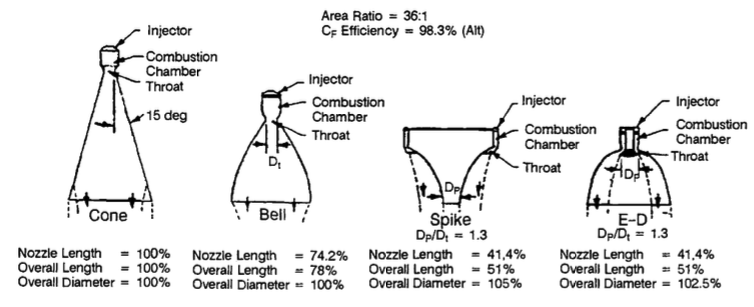
\includegraphics[width=0.7\textwidth]{Figure/nozzles.png}
\end{figure}

\vspace*{-0.5cm}
\section{Scramjet (6$>$M$>$10)}
From the previous analysis in a ramjet, all of the previous evidence points to increasing the burner entry Mach number as the best way to improve performance and efficiency and that the performance gains are proportionally greater for $M_b>1$. Therefore, engines with supersonic burner entry flows are developed called \textit{supersonic combustion ramjets} or \textit{scramjets}. (supersonic combustion is also referred to "\textit{detonation}")\par

However, it has been an engineering problem to achieve supersonic combustion, the main problem is to achieve the \underline{\textbf{mixing of fuel and oxidiser}}. Fundamentally, it is impossible to achieve both supersonic and good mixing at the same time. Also, being able to put in fuel and retain for a finite time for reaction to take place is also a problem. One of the only places that can provide mixing and without generating bow shock is at the \underline{\textbf{boundary layer}}. Problems also arise from:
\begin{itemize}
    \item \textbf{dynamic pressure paradox:} trade-off between featherweight thrust and large drag.
    \item \textbf{Aerothermal heating:} reentry vehicles have strong bow shock for heat dissipation, but bad for performance. 
    \vspace*{-0.2cm}
    \item \textbf{Static start problem}
    \item \textbf{Fuel problem}
\end{itemize}

At high altitude with high flight speed, the intake requires to produce thrust causes the engine to be enormous (fuselage scale), therefore, so far all the design for scramjets looks alike as a half body aircraft, where the aircraft itself is the engine and the compression happens at the lower section. 

\newpage
\section{Rocket}
When reaching h $>$ 90,000 ft, engine starts experiencing oxygen starvation, in which we need to carry our own oxidiser. Rockets are independent of ambient pressure, remain constant designed thrust irrespectively of the altitude, but with poor specific fuel consumption. Th dynamics of the rocket can be modelled as, 
\begin{gather*}
    \sum F = \frac{D}{Dt}(mv)\pmb{e_y} = \dot{m}v+v\dot{v}-\dot{m}u\hspace*{0.4cm}\Rightarrow\hspace*{0.4cm}-mg = \dot{m}u_{rel}+m\dot{v}\\[0.2cm]
    \boxed{v = v_0-u_{rel}\ln\Big(1-\frac{\dot{m}}{m_0}t\Big)-gt}
\end{gather*}
And for multi-stage rockets, the velocity during final stage is
\begin{gather*}
    \boxed{v = u_{rel}\ln\Big(\frac{m_0}{m}\Big) + u_{rel}\sum_{i=1}^{n-1}\ln\Bigg(1-\frac{\dot{m}}{m_0}t\Bigg)-gt}
\end{gather*}
In order to characterise rocket fuels the performance, \textbf{specific impulse} $I_{sp}$ is typically used and has the units of second. 
\begin{gather*}
    I_{sp} = \frac{T}{\dot{m}g}
\end{gather*}

\vspace*{-0.3cm}
\subsection{Cold-gas jets}
can be treated like converging-diverging nozzle with a specified upstream stagnation pressure. gas exiting is inert and process is reasonably isentropic. It is mostly used for RCS, simple, low-interference but very inefficient.

\vspace*{-0.3cm}
\subsubsection{"Hot-gas" jets}
Highly exothermic decomposition of monopropellant liquid hydrazine ($N_2H_4$) when sprayed through an iridium catalyst. Hydrazine decomposes into nitrogen and hydrogen gas, therefore \underline{\textbf{NO oxidiser}} is required as no combustion takes place. However, hydrazine is highly corrosive, toxic and unstable. 

\subsection{Pressure-fed liquid fuel rocket motor}
Inert gas (like helium) is used to pressurise propellant tanks, so no pumps are required. Fuel and oxidiser in pressure-fed systems are usually hypergolic\footnote{components spontaneously ignite when they come into contact with each other} (i.e. monomethyl hydrazine and nitrogen tetroxide) 
\begin{figure}[H]
    \centering
    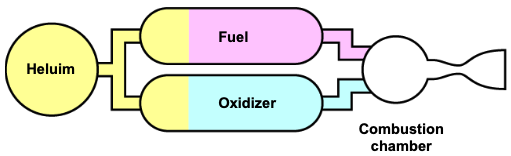
\includegraphics[width=0.5\textwidth]{Figure/pressure-fed.png}
\end{figure}

\vspace*{-0.3cm}
\subsection{Solid-fuel rocket motor}
Fuel and oxidiser combined in a \textbf{solid matrix}, fuel tank IS the combustion chamber. there are generally two main types of propellants. (1) \textbf{Single-based} propellants and (2) \textbf{Composite} propellants. 
\begin{itemize}
    \item \textbf{Fuel:} Aluminium (very small mass fraction)
    \item \textbf{Oxidiser:} Ammonium perchlorate (NH$_4$ClO$_4$, lot of oxygen molecules easily to break off), which constitutes most of the mass of the propellant. (won't ignite at atmospheric pressure)
    \item \textbf{Fuel/Binder:}  Hydroxyl-terminated polybutadiene (HTPB), a synthetic rubber (tyres material).
\end{itemize}
Most of the propellant/fuel only burn at high pressure, therefore, high pressure needs to be created inside the combustion chamber. Once solid motor has been ignited it \textbf{cannot be turned off}, though space shuttle solid motors was equipped with Range-safety system (RSS) that splitting the combustion chamber wall open to release high pressure to stop ignition,

\subsection{Turbopumps}
Large liquid-fuel rockets extract some energy from the expansion of the working fluids, and use this energy to drive the massive fuel pumps.

\begin{multicols}{4}
\subsubsection*{Expansion Turbopumps}
Liquid fuel is vaporised by passing through nozzle, work is extracted from the increase in pressure to drive to pumps. 
\begin{figure}[H]
    \centering
    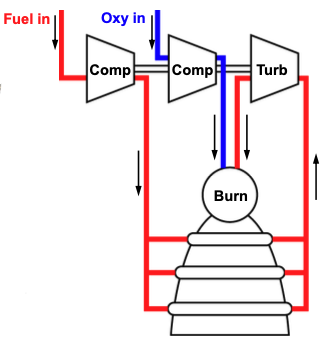
\includegraphics[width=0.28\textwidth]{Figure/turbopump1.png}
\end{figure}

\subsubsection*{Gas-generator turbopumps}
A small amount of fuel is burned separately, and the work to drive the pumps is extracted from the the exhaust. Due to the vented exhaust, some of the potential thrust is lost. 
\begin{figure}[H]
    \centering
    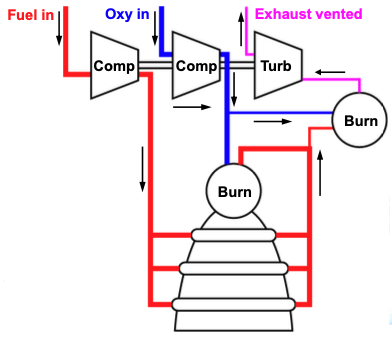
\includegraphics[width=0.27\textwidth]{Figure/turbopump.png}
\end{figure}

\subsubsection*{Staged-combustion turbopump}
The fuel is partially combusted, and work is extracted from the mix of remaining fuel and exhaust.
\vspace*{2cm}
\begin{figure}[H]
    \centering
    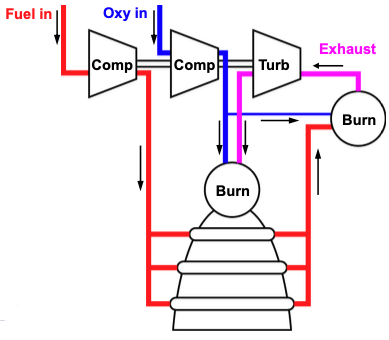
\includegraphics[width=0.27\textwidth]{Figure/staged1.png}
\end{figure}

% \vspace*{1cm}
\subsubsection*{Aspiration turbopump}
cryogenic fuel (LH$_2$/LOX) is used to condense ambient air; this is mixed with additional oxidizer as required. Oxidizer flow can be adjusted depending on availability of atmospheric air. Dramatically improved fuel weight / total weight ratio 
\begin{figure}[H]
    \centering
    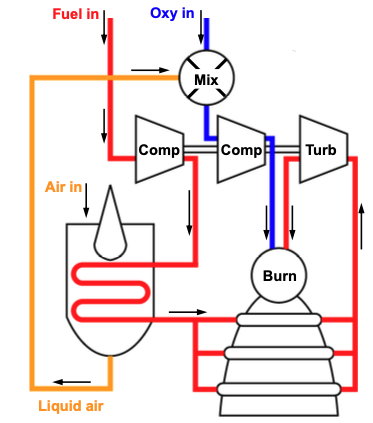
\includegraphics[width=0.25\textwidth]{Figure/aspiration.png}
\end{figure}
\end{multicols}

\subsection{Thermodynamic Analysis on Turbopumps}
The thermodynamic analysis on a conventional expansion turbopump can be done by separating the analysis into fuel and oxygen cycle, to obtain the pressure required at the combustion chamber. 
\begin{gather*}
    W_{turb} = h_3-h_4 = C_pT_3\Bigg(1-\frac{T_4}{T_3}\Bigg) = C_pT_3\Bigg[1-\Bigg(\frac{P_4}{P_3}\Bigg)^{\frac{\gamma-1}{\gamma}}\Bigg]
\end{gather*}

The work generated from the energy of the vapour drives the turbine, thus generating work for both the compressor, therefore, the compressor work should equal to the turbine work,
\begin{gather*}
    W_{turb} = W_{comp1}+W_{comp2} = C_pT_3\Bigg[1-\Bigg(\frac{P_4}{P_3}\Bigg)^{\frac{\gamma-1}{\gamma}}\Bigg]
\end{gather*}
Because the fuel was first passed along through the nozzle, the heat transfer to the fuel from the combustion product can be estimate as following, 
\begin{gather*}
    \frac{Q_{in}}{\dot{m}_{fuel}} = h_3-h_2
\end{gather*}

Though the operation is simple,, the practical design and manufacture of turbopumps is highly complex,
\begin{itemize}
    \item working fluids are cold, bearings and seals are a serious problem, material becomes brittle.
    \item parts are designed to work at supercooled temperatures, parts need to be "pre-cooled"
    \item some rocket fuels are highly corrosive. 
\end{itemize}



\newpage
\section{Hybrid Propulsion}
What if we can find a way to combine all the benefits of a rocket with the other (turbojet, ramjet, scramjet) advantage? Each of them provide specific operating ranges, and pros and cons. This section will be looking into the possibilities of ways to improve different aspects.
\begin{itemize}
    \item \textbf{Turbojet:} are well-developed, mature, reliable tech, but have \underline{low performance ceilings}
    \item \textbf{Ramjets:} are better, but can only work at \underline{high speed and altitude}. 
    \item \textbf{Rockets} are glorified \underline{pipe bombs}. No Mach number or altitude limit. 
    \item \textbf{Scramjets} are still an \underline{experimental} technology.
\end{itemize}

\subsection{Increase Launch Altitude}
If we look back to the rocket equation and express it as a function of altitude ($y=\int vdt$), we can see that the mass of fuel required increases non-linearly with the maximum altitude (takes 50\% of fuel to reach 12\% desired altitude)
\begin{gather*}
    y = (u_{rel}+v_0)t-u_{rel}\Bigg(t-\frac{m_0}{\dot{m}}\Bigg)\ln\Bigg(1-\frac{\dot{m}}{m_0}t\Bigg)-\frac{1}{2}gt^2+y_0
\end{gather*}
What happens if we can increase our initial launch altitude to save the fuel mass required to reach desired altitude? if you can start off only \underline{30\% of the desired altitude}, we can effectively \underline{cut launch mass by 50\%}.

\begin{multicols}{3}
\begin{itemize}
    \item Use a weather balloon
    \item launch from an aeroplane
    \item put wings and turbojets on rocket
    \item nuclear bomb?
    \item Shooting out of a gun
\end{itemize}
\end{multicols}

\subsection{Shooting rocket from a GUN (HARP)}
In order to achieve high pressure inside the gun and high exit velocity, the gun must be enormously long and heavy. If we assume the substance $m$ sits inside the pipe at a distance $L_0+x$ from the end. The pressure at the left is $P$ and at the right (exit direction) is $P_0$, and from pressure difference the equation can be derived as 
\begin{gather*}
    \text{assume}\hspace*{0.4cm}PV^\gamma = P_0V_0^\gamma = C,\hspace*{0.5cm}m\ddot{x} = \frac{P_0L^\gamma}{(L_0+x)^\gamma}-P_0A
\end{gather*} 
Couple factors also dictate the length and the size of the gun. Acceleration decreases with barrel length, which is coupled by pressure to the cross-sectional area or $D^2$. (1) \underline{\textbf{Drag}} increases with $\pmb{D^2}$, (2) \underline{\textbf{Payload capability}} and \underline{\textbf{mass}} increases with $\pmb{D^3}$. This all leads to \textbf{BIGGER} gun. 

\subsection{Oxidiser direct-injection}
Squirt liquid-phase oxidiser directly into combustion chamber with (No longer restricted by Brayton cycle $\eta_{th}>1$)
\begin{itemize}
    \item \underline{\textbf{Pros:}} increase combustor temperature for same fuel flow
    \item \underline{\textbf{Cons:}} (1) carry extra weight for the oxidiser. (2) increasing temperature induces thermal stress and cooling issues. (3) increases the engine complexity and weight. 
\end{itemize}

\subsection{Turbojet pre-cooling}
Instead of spraying oxidiser in to the combustor, we can spray liquid oxygen directly to the inlet are, increasing pressure ratio and reduce the inlet flow temperature. (increasing the ratio $T_b/T_1$).
\begin{itemize}
    \item \underline{\textbf{Pros:}} (1) Overcome oxygen starvation at high altitude. (2) Seriously reduce inlet temperature, increase compressor pressure ratio (and therefore performance)
    \item \underline{\textbf{Cons:}} (1) carry extra weight for the oxidiser. (2) Extremely hard to store cryogenic oxidiser for long haul. (3) Stagnation pressure lose through heat exchangers. 
\end{itemize}

\subsection{Mass-injection pre-compression cooling}
A similar idea is to spray a useful inert coolant (water) into the engine inlet. reduces inlet temperature whilst increases mass flux. The addition of the coolant increases density while decreasing temperature. 
\begin{itemize}
    \item \underline{\textbf{Pros:}} (1) coolant is non-reactive and stable. (2) reduce inlet temperature and increase density - good for performance. (3) HUGE increase in efficiency for most amount of mass injection. (better than LOX)
    \item \underline{\textbf{Cons:}} (1) lots of additional weight. (2) stagnation pressure loss through heat exchangers. (3) Displacing air with steam, and steam doesn't burn.
\end{itemize}
\subsubsection{Thermodynamic Analysis}
Assume using water as pre-compression cooling, objective is to cool down the flow by $5^{\circ}$K to increase the thermo efficiency by 1\%. (heat lost to vapourising the water is about 2000 kJ/kg of water)
\begin{gather*}
    \Delta H_{H_2O} = 2000\cdot\dot{m}_{H_2O};\hspace*{0.3cm}\text{Then for air,}\hspace*{0.3cm}\Delta h = \frac{\Delta H}{\dot{m}_{air}} = \frac{\Delta H_{H_2O}}{\dot{m}_{air}} = 2000\cdot\frac{\dot{m}_{H_2O}}{\dot{m}_{air}} = C_p\Delta T\\[0.2cm]
    \dot{m}_{H_2O} = \frac{C_p\Delta T}{2000}\cdot\dot{m}_{air}
\end{gather*}
the mass flow rate of air can be inferred from the thrust generated, 
\begin{gather*}
    F_T\approx\dot{m}_{air}[u_{exit}-u_{inlet}]
\end{gather*}



\subsection{Increasing Combustion chamber pressure}

\subsubsection{Compressorless compression - pulse jet}
Uses a gradual (but finite) pressure wave rather than a discontinuous shock. Increases combustion pressure increases thermodynamic efficiency of the cycle. operate periodically. 
\begin{figure}[H]
    \centering
    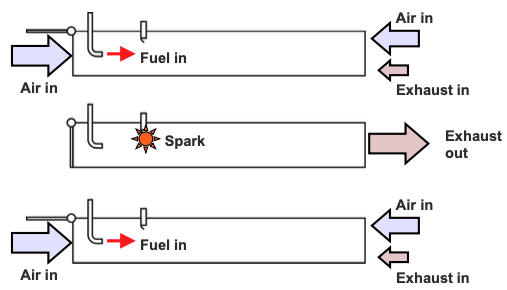
\includegraphics[width=0.5\textwidth]{Figure/pulse.png}
\end{figure}

\vspace*{-0.5cm}
The process where all of the duel-air mix is consumed, leaving only hot combustion products is called \underline{\textbf{\textit{deflagration}}}. If the mix reacts fast enough, the combustion product will expand faster than speed of sound, forming a shock upstream of the exhaust product, this is then called \underline{\textit{\textbf{detonation}}}, which  result in huge increases in pressure relative to just burning, perhaps use detonations in an engine?
\vspace*{0.5cm}
\begin{multicols}{2}
    \begin{figure}[H]
        \centering
        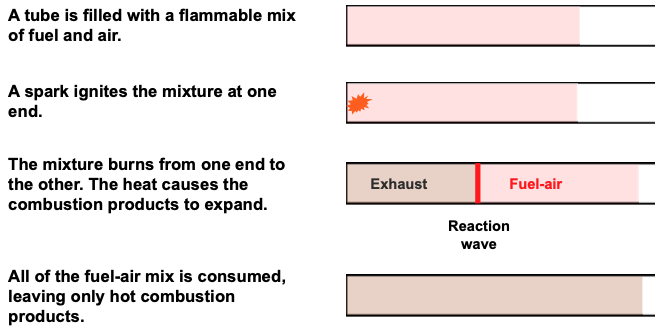
\includegraphics[width=0.43\textwidth]{Figure/deflagration.png}
        \caption[short]{deflagration}
    \end{figure}

    \begin{figure}[H]
        \centering
        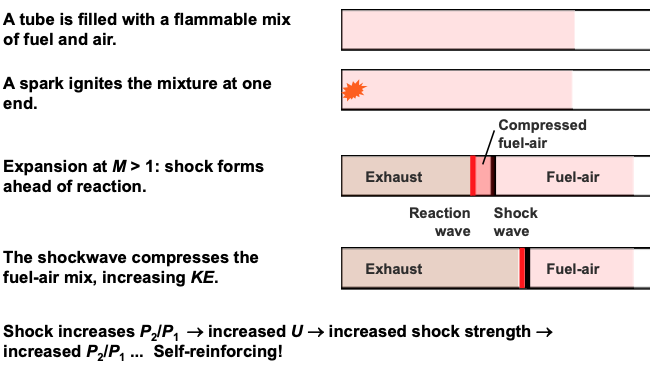
\includegraphics[width=0.43\textwidth]{Figure/detonation.png}
        \caption[short]{detonation}
    \end{figure}
\end{multicols}


\newpage
\section{Detonation}
\textbf{Detonation} is a self-reinforcing process whereby a shock compresses reagents upstream, increasing $\Delta P$ from combustion. Initiated when exhaust gas expand at $M=1$. Expansion rate is a function of rate of combustion, which also depends on mixing. 
\subsection{Governing Equation}
\textbf{Assumptions:} (1) Combustion occurs \textbf{instantaneously} a s a discontinuity. (2) Shock and detonation are coincident. (3) Thermodynamic properties of gas don't change. (3) Pipe area constant.

\begin{figure}[H]
    \centering
    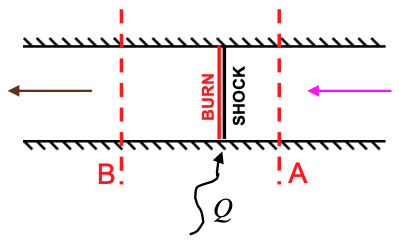
\includegraphics[width=0.4\textwidth]{Figure/detonation scheme.png}
\end{figure}

\vspace*{-0.6cm}
Detonation wave moves from left-to-right. Firstly, from the conservation of mass, momentum we can find an expression of velocity in terms of pressure and density. 
\begin{gather*}
    \begin{split}
        &\text{From mass conserv.:}\hspace*{0.4cm}U_A^2 = \frac{\rho_B}{\rho_A}U_B^2+\frac{P_B-P_A}{\rho_A}\hspace*{0.3cm}\Rightarrow\hspace*{0.3cm}U_A^2 = \frac{1}{\rho_A^2}\Bigg(\frac{P_B-P_A}{\rho_A^{-1}-\rho_B^{-1}}\Bigg)\\
        &\text{From momentum conserv.:}\hspace*{0.4cm}U_B = \frac{\rho_A}{\rho_B}U_A\hspace*{0.3cm}\Rightarrow\hspace*{0.3cm}U_B^2 = \frac{1}{\rho_B^2}\Bigg(\frac{P_A-P_B}{\rho_B^{-1}-\rho_A^{-1}}\Bigg)\\
    \end{split} 
\end{gather*}
This is known as the \textcolor{red}{\textbf{Rayleigh line}}, if we multiply $\rho$ on both sides, and take away the subscript $B$ to treat at any point downstream, and express velocity in terms of Mach number. 
\begin{gather*}
    \rho^2U^2 = \Bigg(\frac{P_A-P}{\rho^{-1}-\rho_A^{-1}}\Bigg)\hspace*{0.4cm}\Rightarrow\boxed{P = -C\rho^{-1}+(P_A+C\rho_A^{-1})}\\[0.2cm]
    \boxed{M_A^2 = \frac{1}{\gamma P_A\rho_A}\Bigg(\frac{P_B-P_A}{\rho_A^{-1}-\rho_B^{-1}}\Bigg)}
\end{gather*}

\vspace*{-0.4cm}
Next, we look at the conservation of energy, which is expressed in the form below consider energy $q$ is added after the shock due to the fuel. By substituting the result from the velocity equation, 
\begin{gather*}
    h_B+\frac{1}{2}U_B^2=h_A+\frac{1}{2}U_A^2+q\hspace*{0.3cm}\Rightarrow\hspace*{0.3cm}h_B-h_A = \frac{1}{2}(U_A^2-U_B^2)+q\\[0.15cm]
    h_B-h_A-q=\frac{1}{2}\Bigg(\frac{1}{\rho_A}+\frac{1}{\rho_B}\Bigg)(P_B-P_A)
\end{gather*}
Then if we substituting $h$ in terms of $P$ and $\rho$, applying ideal gas law and the relation of $C_p = \frac{\gamma R}{\gamma-1}$
\begin{gather*}
    \boxed{\frac{\gamma}{\gamma-1}\Bigg(\frac{P_B}{\rho_B}-\frac{P_A}{\rho_A}\Bigg)-q=\frac{1}{2}\Bigg(\frac{1}{\rho_A}+\frac{1}{\rho_B}\Bigg)(P_B-P_A)}
\end{gather*}

The expression above is called the \textcolor{red}{\textbf{Rankine-Hugoniot relation}}.
\begin{itemize}
    \item For given $P_A,\rho_A,q$, Rankine-Hugoniot relation gives $P$ as function of $1/\rho$
    \item Curve shows possible downstream states. Only points on the curve satisfies mass and momentum.
    \item Rayleigh lines show there are max and min possible values of $\rho^2U^2$. 
\end{itemize}

\begin{multicols}{2}
    \begin{figure}[H]
        \centering
        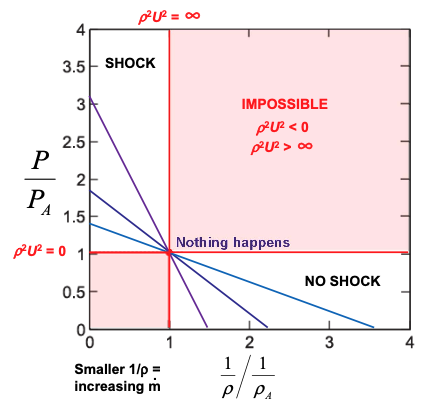
\includegraphics[width=0.36\textwidth]{Figure/rayleigh.png}
    \end{figure}
    \begin{figure}[H]
        \centering
        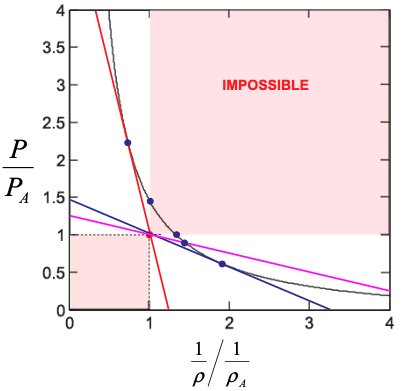
\includegraphics[width=0.36\textwidth]{Figure/RH.png}
    \end{figure}
\end{multicols}

\vspace*{-0.6cm}
To find the relation between $M_A$ and $M_B$, we first need to nondimensionalise and substitute earlier results.
\begin{gather*}
    \begin{split}
        &\text{By substituting}\hspace*{0.2cm}a = \sqrt{\frac{\gamma P}{\rho}},\hspace*{2.3cm}\Rightarrow\hspace*{0.2cm}\frac{2\gamma}{\gamma-1}\Bigg(\frac{P_B}{P_A}\frac{\rho_A}{\rho_B}-1\Bigg)-\frac{q}{a_A^2} = \Bigg(1+\frac{\rho_A}{\rho_B}\Bigg)\Bigg(\frac{P_B}{P_A}-1\Bigg)\\
        &\text{From}\hspace*{0.3cm}M_A^2 = \frac{1}{\gamma P_A\rho_A}\Bigg(\frac{P_B-P_A}{\rho_A^{-1}-\rho_B^{-1}}\Bigg),\hspace*{1cm}\Rightarrow\hspace*{0.2cm}\frac{\rho_A}{\rho_B}=\frac{1}{\gamma M_A^2}\Bigg(1-\frac{P_B}{P_A}\Bigg)+1
    \end{split}\\[0.5cm]
    \boxed{\frac{2\gamma}{\gamma-1}\Bigg[\frac{P_B}{P_A}\Bigg(\frac{1}{\gamma M_A^2}\Bigg[1-\frac{P_B}{P_A}\Bigg]+1\Bigg)-1\Bigg]-\frac{q}{a_A^2}=\Bigg[\Bigg(\frac{1}{\gamma M_A^2}\Bigg[1-\frac{P_B}{P_A}\Bigg]+2\Bigg)\Bigg]\Bigg(\frac{P_B}{P_A}-1\Bigg)}
\end{gather*}

Detonation needs \textbf{shock} for compression, therefore the maximum downstream Mach number is $M_B=1$. This is due to the added energy and combustion, and the fact that the area is constant and without expansion, the flow cannot go supersonic. From conservation of momentum with pressure,
\begin{gather*}
    \frac{P_B}{P_A} = \frac{1+\gamma M_A^2}{1+\gamma M_B^2} = \frac{1+\gamma M_{CJ}^2}{1+\gamma}\hspace*{0.5cm}\text{When}\hspace*{0.3cm}M_B=1\rightarrow M_A = M_{CJ} 
\end{gather*}

The resulting $M_A$ is defined as the \textcolor{red}{\textbf{Chapman-Jouguet}} Mach Number $M_{CJ}$. For detonation to happen, we need to reach $M_{CJ}$ where we can plug this requirement back to the above equation and solve for the Mach number $M_CJ$ for detonation, we can then get
\begin{gather*}
    M_{CJ}^2 = \Bigg((\gamma+1)(\gamma-1)\frac{q}{a_A^2}+1\Bigg)\pm\sqrt{\Bigg((\gamma+1)(\gamma-1)\frac{q}{a_A^2}+1\Bigg)^2-1}
\end{gather*}
Discard the negative solution due to the non-physicality, and using the relation $a = \sqrt{\gamma RT}$ and $C_p = \frac{\gamma R}{\gamma-1}$, we can arrive to the final expression
\begin{gather*}
    \boxed{M_{CJ}^2 =\Bigg((\gamma+1)\frac{q}{C_pT_A}+1\Bigg)+\sqrt{\Bigg((\gamma+1)\frac{q}{C_pT_A}+1\Bigg)^2-1}}
\end{gather*}
\vspace*{-0.3cm}
\begin{figure}[H]
    \centering
    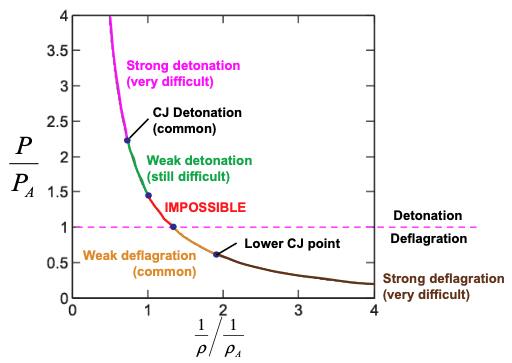
\includegraphics[width=0.5\textwidth]{Figure/MCJ.png}
\end{figure}

\subsection{Detonation analysis}
As an example, let's consider a stoichiometric hydrogen/air mix. 
\begin{gather*}
    \begin{split}
        &\text{For air:}\hspace*{0.3cm}C_p = 1.00\hspace*{0.4cm}\gamma = 1.4\hspace*{0.4cm}f_{FA} = 0.028\\
        &\text{For H}_2:\hspace*{0.3cm}C_p = 14.32\hspace*{0.4cm}\gamma = 1.4.
    \end{split}
\end{gather*}
where $q = f_{FA}\varepsilon$, where $\varepsilon = 120000$ kJ/kg. $C_p$ for hydrogen/air mixtures scale roughly with the relative volumes fo mixed gases, so 
\vspace*{-0.09cm}
\begin{gather*}
    C_p\approx\frac{V_{fuel}C_{p,fuel}+V_{air}C_{p,air}}{V_{fuel}+V_{air}}\approx\Bigg(\frac{m_fR_fT_f}{P_f}C_{p,fuel}+\frac{m_aR_aT_a}{P_a}C_{p,air}\Bigg)\Bigg(\frac{m_fR_fT_f}{P_f}+\frac{m_aR_aT_a}{P_a}\Bigg)^{-1}
\end{gather*}

Since gases are mixed: $P_f = P_a$ and $T_f = T_a$, where $m_f = f_{FA}m_a$.

\vspace*{-0.5cm}
\begin{gather*}
    C_p\approx\frac{f_{FA}m_aR_fC_{p,fuel}+m_aR_aC_{p,air}}{f_{FA}m_aR_f+m_aR_a}\approx\boxed{\frac{f_{FA}R_fC_{p,fuel}+R_aC_{p,air}}{f_{FA}R_f+R_a}} = 4.905\text{ J/Kg}^{\circ}\text{K},\hspace*{0.4cm}\\[0.2cm]
    \text{Similarly,}\hspace*{0.4cm}\gamma_f = \frac{f_{FA}R_f\gamma_f+R_{air}C_{p,air}}{f_{FA}R_f+R_{air}}\\[0.2cm]
    \because\hspace*{0.2cm}R_f = C_{p,fuel}\frac{\gamma_f-1}{\gamma_f} = 4091\text{ J/Kg}^{\circ}\text{K}\hspace*{0.5cm}
\end{gather*}
Then, at say $T = 300$ K,
\begin{gather*}
    M_{CJ}^2 = \Bigg((\gamma+1)\frac{q}{C_pT_A}+1\Bigg)+\sqrt{\Bigg((\gamma+1)\frac{q}{C_pT_A}\Bigg)^2-1}\hspace*{0.3cm}\Rightarrow\hspace*{0.3cm}\boxed{M_{CJ} \approx4.22}
\end{gather*}

\subsection{Humphrey cycle}
The cycle efficiency can be expressed as, we also need to find expression for the expansion temperature ratio $T_4/T_1$
\begin{gather*}
    \eta_{cycle} = 1-\frac{h_4-h_1}{\Delta h_{burn}}=1-\frac{C_p(T_4-T_1)}{q} = 1-\frac{C_pT_1}{q}\Bigg(\frac{T_4}{T_1}-1\Bigg)
\end{gather*}

\begin{multicols}{2}
    \begin{figure}[H]
        \centering
        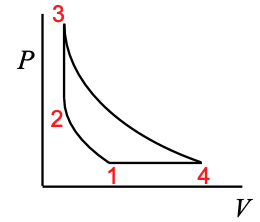
\includegraphics[width=0.2\textwidth]{Figure/PV.png}
    \end{figure}
    \begin{figure}[H]
        \centering
        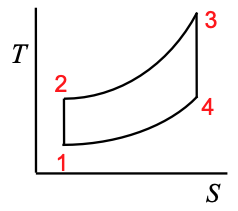
\includegraphics[width=0.2\textwidth]{Figure/TS.png}
    \end{figure}
\end{multicols}
\vspace*{-0.5cm}
From the definition of entropy, and $h = e+P\nu$
\begin{gather*}
    dq = Tds = de+Pd\nu\hspace*{0.3cm}\Rightarrow\hspace*{0.3cm}ds = \frac{1}{T}dh-\frac{\nu}{T}dP\hspace*{0.3cm}\Bigg(\because\frac{\nu}{T} = \frac{1}{\rho T}=\frac{R}{P} = \frac{\gamma-1}{\gamma}\frac{C_p}{P}\Bigg)\\[0.2cm]
    \Rightarrow\hspace*{0.3cm}\int_{1}^{4}ds = C_p\int_{1}^{4}\frac{dT}{T}-C_p\frac{\gamma -1}{\gamma}\int_{1}^{4}\frac{dP}{P}\hspace*{0.3cm}\Rightarrow\hspace*{0.3cm}\frac{s_4-s_1}{C_p}=\ln\Bigg(\frac{T_4}{T_1}\Bigg)-\frac{\gamma-1}{\gamma}\ln\Bigg(\frac{P_4}{P_1}\Bigg)
\end{gather*}
If we substitute this back to our $\eta$ expression for temperature, and make the assumption that $P_1=P_4$, the cycle efficiency is then express as the following. If we constraint ourselves to the \textbf{efficiency before and after the shock}
\begin{gather*}
    \begin{split}
        \eta_{cycle} &= 1-\frac{C_pT_1}{q}\Bigg[\exp\Bigg(\frac{s_3-s_2}{C_p}\Bigg)-1\Bigg]\\[0.2cm]
        &= 1-\frac{C_pT_1}{q}\Bigg(\exp\Bigg[\ln\Bigg(\frac{T_3}{T_2}\Bigg)-\frac{\gamma-1}{\gamma}\ln\Bigg(\frac{P_3}{P_2}\Bigg)\Bigg]-1\Bigg)
    \end{split}
\end{gather*}
The combustion takes place across the control volume, and the pressure ratio and temperature ratio are expressed as the Following
\begin{gather*}
    \frac{P_B}{P_A}=\frac{1+\gamma M_{CJ}^2}{1+\gamma}\hspace*{0.6cm}\frac{T_B}{T_A}=\frac{1}{M_{CJ}^2}\Bigg(\frac{1+\gamma M_{CJ}^2}{1+\gamma}\Bigg)^2
\end{gather*}
Then if we substitute all the above, we can arrive to the final expression of the cycle efficiency
\begin{gather*}
    \boxed{\eta_{cycle} = 1-\frac{C_pT_1}{q}\Bigg(\frac{1}{M_{CJ}^2}\Bigg(\frac{1+\gamma M_{CJ}^2}{1+\gamma}\Bigg)^{\frac{\gamma+1}{\gamma}}-1\Bigg)}
\end{gather*}
However, the analysis are crude approximation where our estimated C-J Mach number is a bit low.
\begin{itemize}
    \item $C_p$ approximation was very crude. 
    \item C-J model itself is simplistic.
    \item The exhaust certainly does not have the same thermodynamic properties as the fuel/air mix
    \item Approximations worsen for heavy hydrocarbons. 
\end{itemize}
There are three main observation we can make on using detonation as oppose to gas-turbines. 
\begin{enumerate}
    \item For the same temperature ratio, detonations would be much \textbf{more efficient} than a gas turbine especially at \underline{lower temperature ratios}.
    \item Efficiency is a strong function of $q/C_pT_1$, so the \textbf{better the fuel}, the \textbf{more efficient} the engine
        \begin{gather*}
            \begin{split}
            \text{(Brayton cycle)}\hspace*{0.5cm}\eta_{cycle} &= \frac{C_pT_1}{f{FA}\varepsilon}\Bigg(\frac{T_2}{T_1}-1\Bigg)\Bigg(\eta_c\eta_e\Bigg(1+\frac{T_1}{T_2}\frac{f_{FA}\varepsilon_1}{C_pT_1}\Bigg)-1\Bigg)\\
            &= \frac{C_pT_1}{f{FA}\varepsilon}\Bigg(\frac{T_2}{T_1}-1\Bigg)\Bigg(1+\frac{T_1}{T_2}\frac{f_{FA}\varepsilon_1}{C_pT_1}-1\Bigg)\\
            &= \frac{C_pT_1}{f{FA}\varepsilon}\frac{f_{FA}\varepsilon_1}{C_pT_1}\Bigg(\frac{T_2}{T_1}-1\Bigg)\Bigg(\frac{T_1}{T_2}\Bigg)\\
            & = \boxed{1-\frac{T_1}{T_2}}\\
            \text{(Humphrey cycle)}\hspace*{0.5cm}\eta_{cycle} &= 1-\frac{C_pT_1}{q}\Bigg(\frac{1}{M_{CJ}^2}\Bigg(\frac{1+\gamma M_{CJ}^2}{1+\gamma}\Bigg)^{\frac{\gamma+1}{\gamma}}-1\Bigg)\\
            &\approx1-\frac{C_pT_1}{q}\Bigg(\frac{(M_{CJ}^2)^{\frac{\gamma+1}{\gamma}}}{M_{CJ}^2}\Big(\frac{\gamma}{1+\gamma}\Big)^{\frac{\gamma+1}{\gamma}}-1\Bigg)\\
            &\approx\boxed{1-\frac{C_pT_1}{q}(0.397M_{CJ}^{1.43}-1)}
            \end{split}
        \end{gather*}
    \item There is a minimum value of $q/C_pT_1$ below which the detonation won't work: the case where $\pmb{\eta} = 0$.
        \begin{gather*}
            q_{min} = 0\hspace*{0.3cm}\text{when}\hspace*{0.3cm}M_{CJ} = 1
        \end{gather*}
\end{enumerate}

\newpage
\subsection{Pulse-Detonation Engines (PDE)}
\subsubsection*{Forcing-deflagration-to-detonation transition (DDT)}
\begin{multicols}{2}
    \begin{itemize}
        \item \textbf{Material stress:} it is literally a bomb, structure must withstand loads but provide good thrust/weight.
        \item \textbf{Noise:} The high Mach number shocks spitting out the tube will generate enormous amounts of acoustic noise compared to a turbojet. 
        \item \textbf{mechanical valve:} The thrust generated is enormous only when engine fires. The average thrust will be a function of the \textbf{frequency} of the firing, which is limited by valve action. 
    \end{itemize}
    \begin{figure}[H]
        \centering
        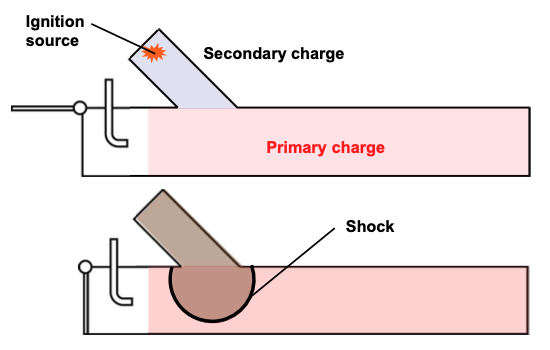
\includegraphics[width=0.5\textwidth]{Figure/DDT.png}
    \end{figure}
\end{multicols}
\subsubsection*{Continuous detonation wave engine (CDE)}
\begin{multicols}{2}
    \begin{itemize}
        \item \textbf{Pros:}
            \begin{itemize}
                \item Frequency of Tens of kHz continuous smooth operation. No complex moving parts, only need to ignite once. 
            \end{itemize}
        \item \textbf{Cons:}
            \begin{itemize}
                \item Incoming fuel/air will always mix with exhaust products, lowering combustion efficiency, causing Detonation wave slower than C-J Mach number ($q$ is lower than pure fuel/air)
                \item Need pre-compressed fuel/air
            \end{itemize}
    \end{itemize}
    \begin{figure}[H]
        \centering
        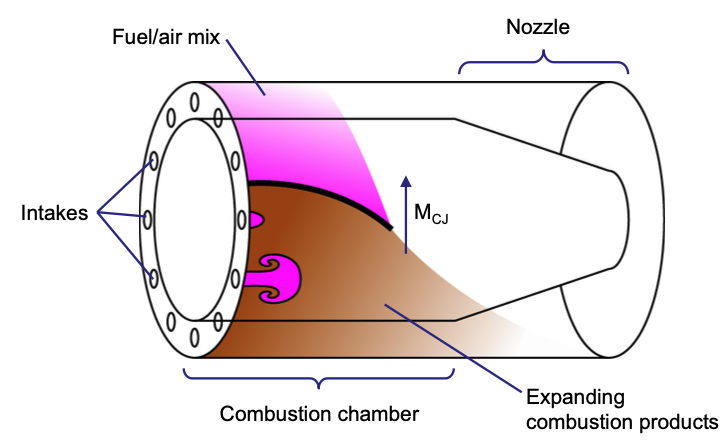
\includegraphics[width=0.55\textwidth]{Figure/CDE.png}
    \end{figure}
\end{multicols}
%%%%%%%%%% %%%%%%%%%%

\end{document}
 